\documentclass[tikz,border=10pt]{standalone}

\begin{document}
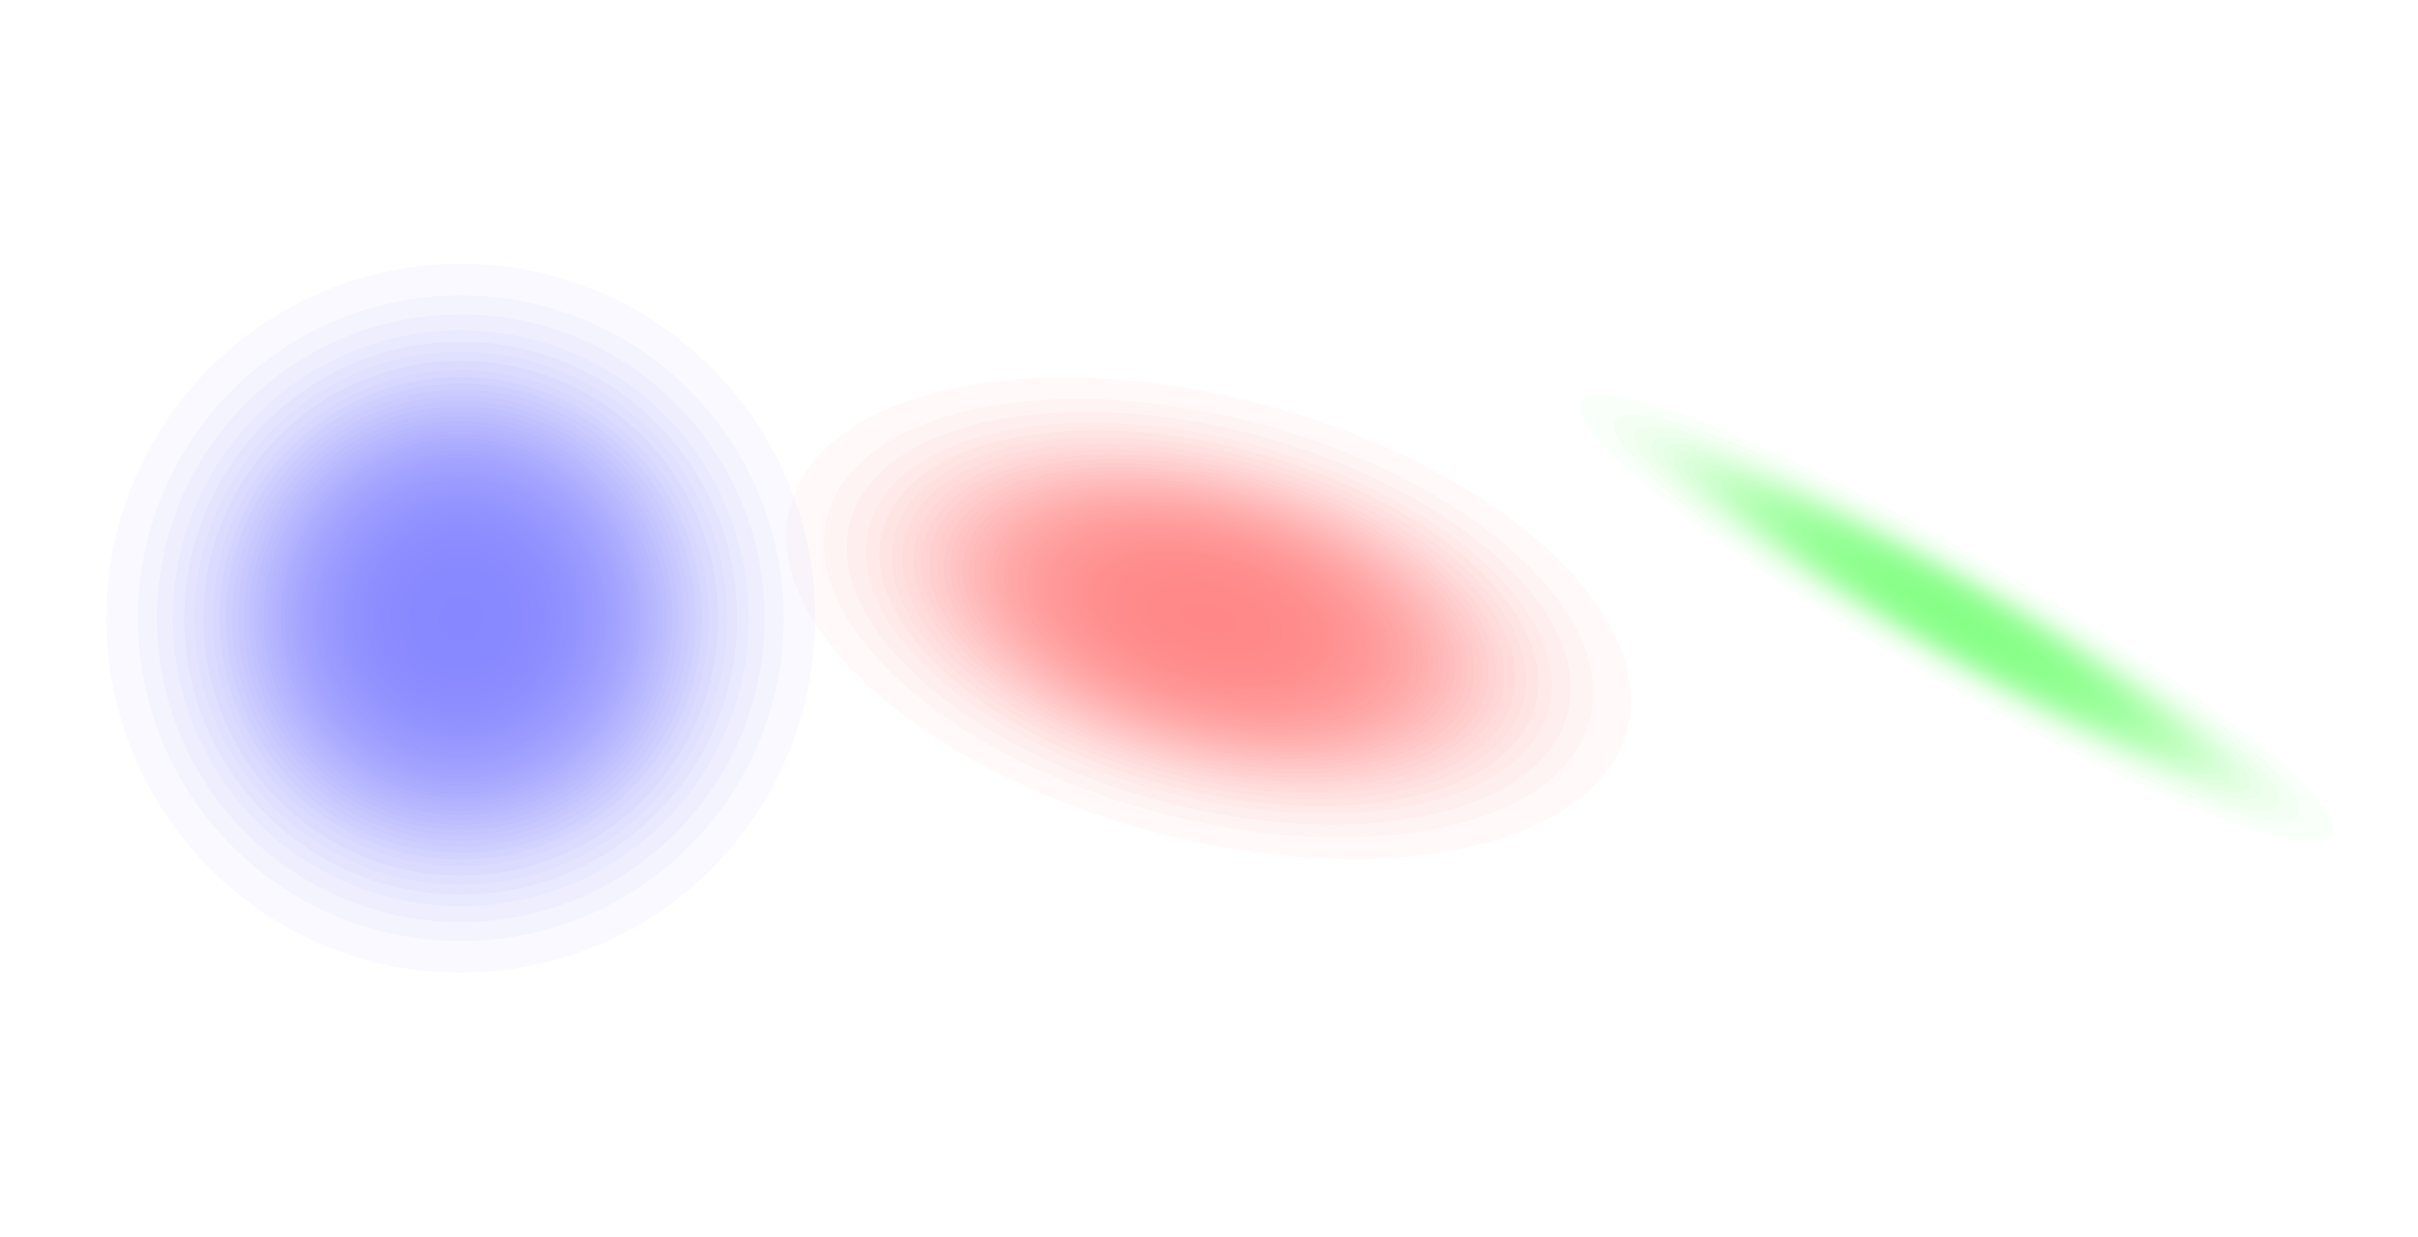
\begin{tikzpicture}[x=1cm,y=1cm]

% Define overall image dimensions and canvas size (ratio 2:1 -> 30x15)
% Using \path keeps the background completely transparent
\path (0,0) rectangle (30,15);

% Center coordinates for the three shapes (evenly spaced)
\coordinate (blueCenter)  at (5.5, 7.5);
\coordinate (redCenter)   at (15, 7.5);
\coordinate (greenCenter) at (24.5, 7.5);

% Define maximum radii for the shapes (at 3 sigma, opacity drops to ~0)
% Blue Sphere (Isotropic Gaussian)
\def\bluemaxrx{4.5} \def\bluemaxry{4.5}
% Red Cigar (Moderately Anisotropic)
\def\redmaxrx{5.5} \def\redmaxry{2.8}
% Green Needle (Highly Anisotropic)
\def\greenmaxrx{5.5} \def\greenmaxry{0.8}

% Define rotation angles
\def\redrot{-15}
\def\greenrot{-30}

% --- True Gaussian Drawing Function ---
% [#1] Number of layers (defaults to 60 for a super smooth gradient)
% #2   Center coordinate name
% #3   Max x-radius (~3 standard deviations)
% #4   Max y-radius
% #5   Rotation (degrees)
% #6   Base color
\newcommand{\drawfuzzygaussian}[6][60]{
    % Calculate constant alpha per layer to reach 0.95 opacity at the absolute core
    % Max Alpha = 1 - (1 - opac)^N = 0.95  =>  opac = 1 - exp(-3.0 / N)
    \pgfmathsetmacro{\opac}{ 1 - exp(-3.0 / #1) }

    \foreach \i in {1,...,#1} {
        % To achieve a true Gaussian opacity profile (bell curve),
        % space the layer radii non-linearly using the inverse Gaussian CDF:
        % r_i = sqrt( ln(i / N) / ln(1 / N) )
        % This forces the visual density to fade exactly like a normal distribution.
        \pgfmathsetmacro{\sizefact}{ sqrt( max(0, ln(\i / #1) / ln(1 / #1)) ) }
        
        \fill[#6, opacity=\opac, rotate around={#5:(#2)}] 
            (#2) ellipse ({\sizefact * #3} and {\sizefact * #4});
    }
}

% --- Draw Shapes ---

% Shape 1: Blue Sphere (Isotropic Gaussian)
\drawfuzzygaussian{blueCenter}{\bluemaxrx}{\bluemaxry}{0}{blue!50}

% Shape 2: Red Cigar (Medium Anisotropy)
\drawfuzzygaussian{redCenter}{\redmaxrx}{\redmaxry}{\redrot}{red!50}

% Shape 3: Green Needle (High Anisotropy)
\drawfuzzygaussian{greenCenter}{\greenmaxrx}{\greenmaxry}{\greenrot}{green!50}

\end{tikzpicture}
\end{document}